\chapter{Arhitectura programului}

Scopul extensiei create este de prelua un fișier PDF încărcat de profesor într-un formular din Moodle și de a genera automat module de învățare și teste grilă, teste cu patru variante de
răspuns și doar una corectă, pe baza informațiilor din fișier. Mediul de dezvoltare folosit este XAMPP, cu un server Apache, limbajul de programare PHP, o bază de date MariaDB, și
platforma Moodle instalată local. Generarea conținutului educațional pe baza materialului încărcat se face cu ajutorul API-ului Gemini de la Google, care oferă un model de inteligență 
artificială capabil să extragă și să reformuleze text pentru a genera module de învățare și să creeze întrebări cu un singur răspuns corect pentru testele ce faciliteaza trecerea individului 
la următorul nivel.  

\section{Arhitectura generală}

Arhitectura sistemului utilizează modelul client-server. Clientul este reprezentat de interfața Moodle, iar aceasta diferă în funcție de rolul utilizatorului. Pentru profesor, interfața 
permite încarcarea fișierului PDF și vizualizarea modulelor de învățare înainte de a le valida și publica. Pentru student, interfața permite vizualizarea modulelor de învățare și a testelor 
generate. Serverul este aplicația Moodle încărcată local pe care este instalată extensia. Backend-ul extensiei se ocupă cu preluarea fișierului PDF, gestionarea permisiunilor de acces, 
încărcarea informațiilor în baza de date și comunicarea cu API-ul Gemini, folosit pentru generearea conținutului din cadrul modulelor și a testelor.

\begin{figure}[ht]
    \centering
    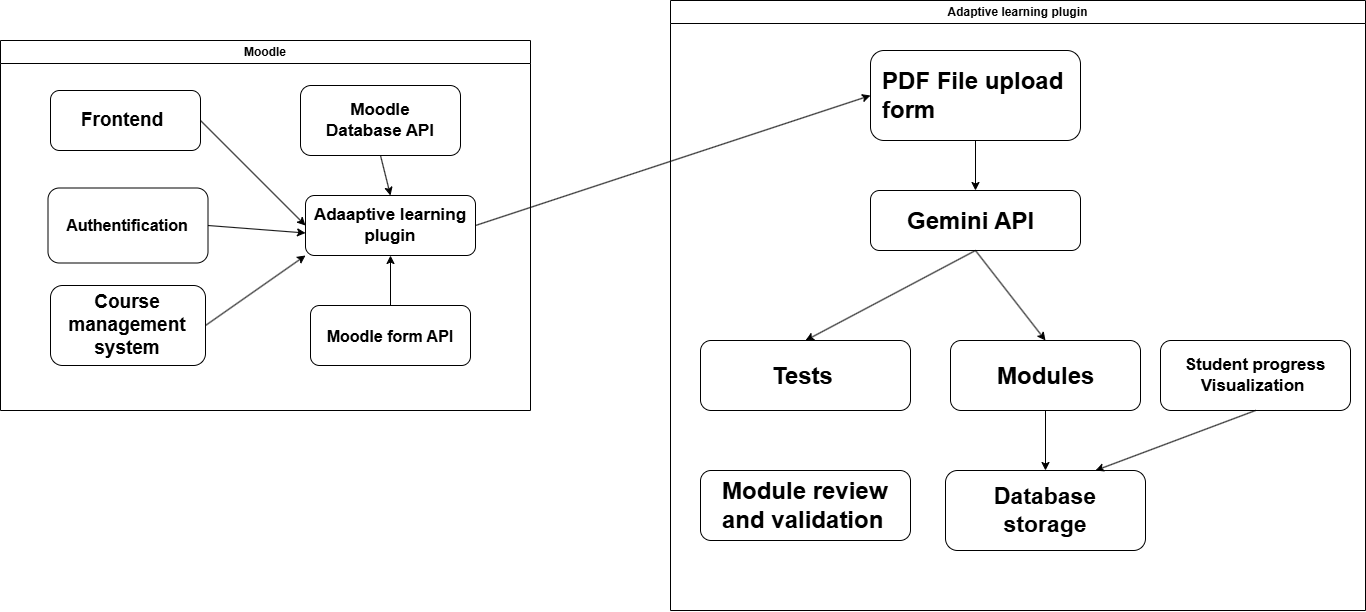
\includegraphics[width=0.8\textwidth]{images/LicentaArchitectureDiagram.png}
    \caption{Arhitectura generală a extensiei}
    \label{fig:arch_diagram}
\end{figure}

\section{Tehnologiile utilizate}

\subsection{Moodle}

Moodle este sistemul de management al învățării (LMS) pentru care este concepută această extensie. Moodle este o aplicație web scrisă în PHP [3], de tip open-source, care are ca scop 
oferirea unui mediu unificat de învățare profesorilor și studenților. Aceasta a luat naștere dintr-un proiect de cercetare doctorală (PhD) condus de Martin Dougiamas, cu ajutorul lui 
Peter C. Taylor, la Curtin University of Technology. Scopul principal al proiectului de cercetare a fost de a explora cum software-ul de internet poate sprijini cu succes epistemologii 
de predare și învățare bazate pe construcționismul social. Întrebarea principală a cercetării a fost clară: ce tipuri de structuri web și interfețe ajută sau, dimpotrivă, împiedică 
implicarea activă a participanților într-un dialog reflexiv, într-o comunitate de învățare? Accentul a fost pus pe sprijinirea lecturii deschise, a reflecției critice și a unei scrieri 
constructive, care să pornească din experiențele personale ale cursanților. Pe baza acestor observații, dezvoltarea platformei Moodle este orientată constant de această analiză, 
fiind gândită ca un instrument care sprijină și îmbunătățește procesele de învățare reflexivă în comunitate. [8]

Acest model open-source permite ca modificările făcute de utilizatori să fie adesea integrate în proiectul principal, permițând 
software-ului să evolueze conform valorilor comunității de utilizatori. Designul Moodle a fost gândit specific pentru a fi compatibil, flexibil și ușor de modificat. 
Este scris în limbajul PHP și este construit modular, utilizând tehnologii comune. Această abordare modulară a fost adoptată inițial pentru a permite modificarea 
rapidă a interfețelor ca răspuns la analiză și interese de cercetare, dar acum permite și altor programatori să modifice și să extindă codul. [8] Adaptibilitatea este o caracteristică
importantă pentru cei ce aleg să folosească Moodle. Spre deosebire de software-ul restricționat de licențe care limitează personalizarea, Moodle permite accesul la codul sursă și 
modificarea acestuia, această flexibilitate fiind văzută ca un mare avantaj. Capacitatea de a personaliza Moodle a fost un motiv pentru adoptare la instituții precum Otago Polytechnic 
din Noua Zeelandă și  Dublin City University (DCU).[9]

Distribuția Moodle are trei componente principale: codul sursă ce rulează pe un server web, o baza de date relațională (MariaDB) destinată stocării datelor și un spațiu de depozitare pentru
toate fișierele folsoite (folderul moodledata). Cursurile, activitățile și resursele sunt stocate în baza de date, iar extensiile instalate sunt stocate în folderul moodledata. Extensia 
creată intră în această categorie ca un modul de activitate. Moodle definește un modul de activitate ca fiind o extensie în care studentul interacționează cu alți studenți sau cu 
profesorul. Într-o activitate, studenții pot contribui direct la ceva propus de profesor, cum ar fi o resursă în forma unui fișier sau a unei pagini web.[3] Extensia este formată dintr-un
set de fișiere PHP, precum version.php, lib.php, view.php,  etc. și fișiere CSS și JavaScript pentru stilizare și interactivitate. Moodle apelează funcțiile extensiei în momentul în care
utilizatorul accesează pagina acesteia în interfața web. Prin utilizarea API-ului Moodle, extensia are parte de mecanisme standard pentru gestionarea bazei de date, controlul accesului
și a permisiunilor și de integrare, instalare și actualizare ușoară.

\subsection{XAMPP}

Pentru dezvoltarea, testarea locală a extensiei și pentru rularea Moodle, a fost utilizat XAMPP. XAMPP este un pachet software gratuit care conține Apache, MariaDB, PHP și 
Perl, „XAMPP este cel mai popular mediu de dezvoltare PHP”[4]. În contextul dezvoltării extensiei, Apache servește ca server web pentru aplicația Moodle și răspunde la cererile HTTP ale
utilizatorilor. Am ales XAMPP deoarece facilitează o configurare rapidă și simplă a mediului de dezvoltare deoarece nu este necesară instalarea separată a fiecărei componentă în parte.

\subsection{MariaDB}

MariaDB este sistemul de baze de date relațional folosit pentru stocarea datelor aplicației Moodle. MariaDB a fost creat inițial ca „fork al MySQL”, menținând compatibilitatea cu 
acesta la nivel de protocol și dialect SQL[4].